% BAYZYO-2026 poster — 70x100 cm portrait, 2 cm margins. Compile: xelatex poster.tex
% White backgrounds throughout (print-economical); colored accents only.
\documentclass{article}

\usepackage[paperwidth=70cm,paperheight=100cm,margin=2cm]{geometry}
\usepackage{fontspec}
\usepackage{ragged2e}
\usepackage{xcolor}
\usepackage{graphicx}
\usepackage{adjustbox}
\usepackage{array}
\usepackage{booktabs}
\usepackage{amssymb}
\usepackage{enumitem}
\usepackage[most]{tcolorbox}

% ---- Arial-like sans (spec: Arial/Verdana/Times) ----
\setmainfont{Nimbus Sans}
\newfontfamily\monofont{DejaVu Sans Mono}

% ---- theme ----
\definecolor{pblue}{RGB}{15,60,110}
\definecolor{pteal}{RGB}{0,120,135}
\definecolor{pgold}{RGB}{140,98,8}

% ---- font-size roles (spec point ranges) ----
\newcommand{\titlefont}{\fontsize{48}{56}\bfseries}
\newcommand{\subfont}{\fontsize{28}{34}\selectfont}
\newcommand{\authorfont}{\fontsize{32}{40}\bfseries}
\newcommand{\addrfont}{\fontsize{26}{32}\selectfont}
\newcommand{\badgefont}{\fontsize{27}{33}\bfseries}
\newcommand{\headfont}{\fontsize{28}{34}\bfseries}
\newcommand{\bodyfont}{\fontsize{25}{31}\selectfont}
\newcommand{\smallfont}{\fontsize{22}{27}\selectfont}
\newcommand{\reffont}{\fontsize{15}{19}\selectfont}

\setlength{\parindent}{0pt}

% ---- section panel: WHITE body, blue frame + blue header bar ----
\newtcolorbox{panel}[1]{
  enhanced, breakable=false,
  colback=white, colframe=pblue, boxrule=1.4pt, arc=6pt,
  left=11pt, right=11pt, top=6pt, bottom=7pt,
  fontupper=\bodyfont\justifying,
  title={#1}, fonttitle=\headfont, coltitle=white, colbacktitle=pblue,
  toptitle=4pt, bottomtitle=4pt, lefttitle=11pt,
  before skip=0pt, after skip=9pt,
}

\newcommand{\keyval}[1]{\textcolor{pteal}{\bfseries #1}}
\setlist[itemize]{leftmargin=1.25em, itemsep=3pt, topsep=3pt, parsep=0pt}
\newcommand{\figcap}[1]{\vspace{-1pt}{\smallfont #1}}

\pagestyle{empty}

\begin{document}
\centering

% =========================== TITLE BANNER (white) ===========================
\begin{tcolorbox}[enhanced, colback=white, colframe=pblue, boxrule=2.4pt,
  arc=10pt, left=24pt, right=24pt, top=11pt, bottom=11pt, width=\textwidth]
\centering
{\titlefont\color{pblue} PERCEIVE--REASON--CODE}\\[5pt]
{\subfont\color{black} Active Perception for Document VQA}\\[11pt]
{\authorfont\color{black} \underline{Barış Deniz Sağlam}}\\[5pt]
{\addrfont\color{black} Middle East Technical University \,\textbullet\, Informatics Institute \,\textbullet\, PhD Student}\\[11pt]
\begin{tcolorbox}[enhanced, colback=pgold, colframe=pgold, boxrule=0pt, arc=6pt,
  left=18pt,right=18pt,top=6pt,bottom=6pt, width=0.86\textwidth, halign=center]
\color{white}\badgefont ICDAR 2026 DocVQA Challenge \,\textbullet\, JOINT WINNER \,\textbullet\, 8--35B PARAMETER TIER
\end{tcolorbox}
\end{tcolorbox}

\vspace{4pt}
\raggedright

% =========================== LEFT BLOCK (2 cols) + RIGHT SIDEBAR ===========================
\begin{minipage}[t]{0.655\textwidth}\vspace{0pt}
% ---- HERO: method figure spanning the two left columns ----
\begin{tcolorbox}[enhanced, colback=white, colframe=pblue, boxrule=1.4pt, arc=6pt,
  left=11pt, right=11pt, top=6pt, bottom=8pt, width=\linewidth,
  title={THE METHOD IN ONE TRACE}, fonttitle=\headfont, coltitle=white,
  colbacktitle=pblue, toptitle=4pt, bottomtitle=4pt, lefttitle=11pt]
\centering
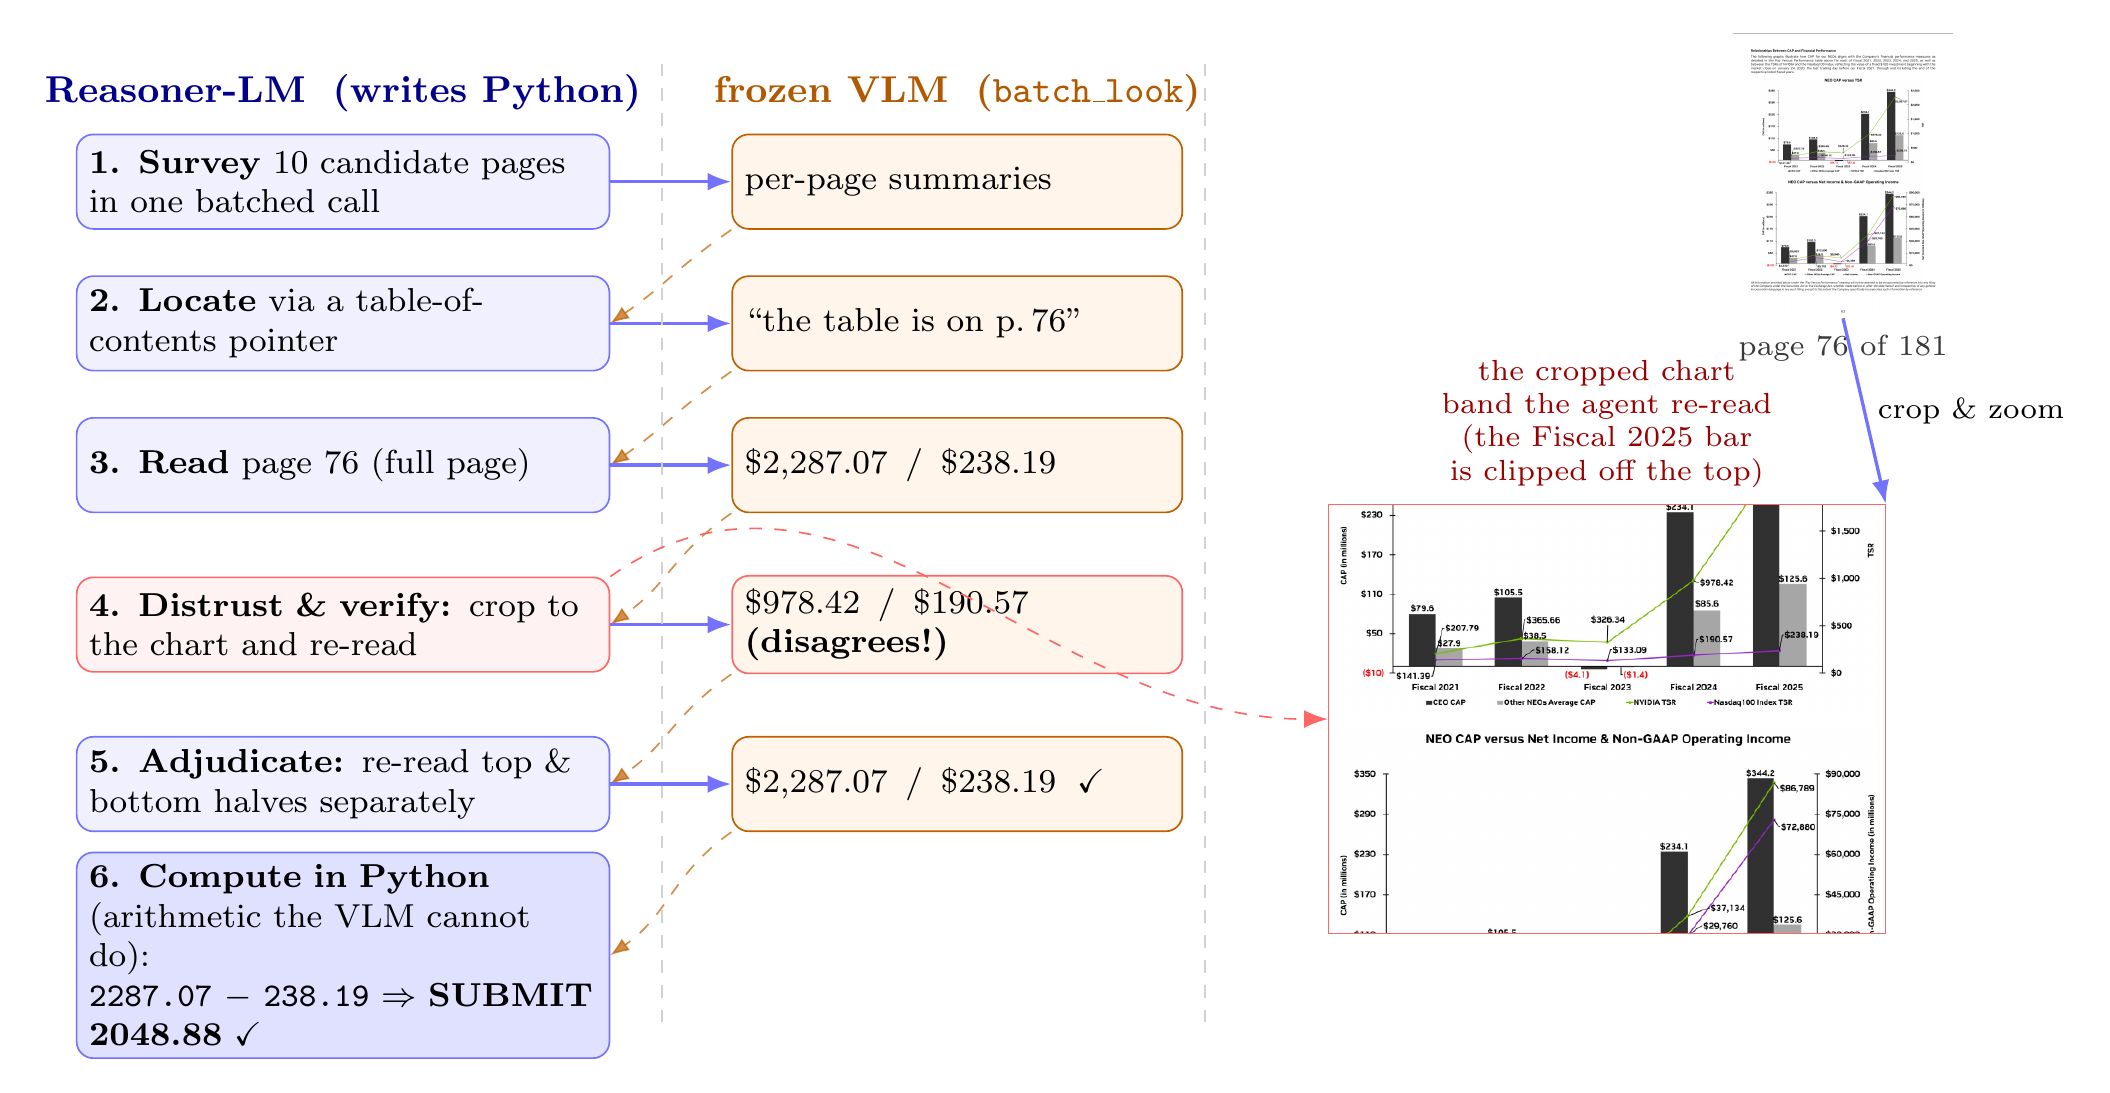
\includegraphics[width=0.99\linewidth]{figures/trajectory-1.png}\\[3pt]
\begin{minipage}{0.98\linewidth}\justifying
\figcap{\textbf{Fig.~1.} \keyval{Perceive--Reason--Code} on a 181-page report. The
reasoner-LM writes Python that calls the \keyval{Perceiver} (VLM) on regions it
chooses: it \keyval{surveys} pages, \keyval{locates} the table,
\keyval{distrusts} a full-page read, re-reads a tighter \keyval{crop} that
disagrees, adjudicates, and \keyval{computes} the answer in Python --- finding
\emph{across} pages and reading \emph{within} one. The crop-verify catches a wrong
number a single read would have submitted.}
\end{minipage}
\end{tcolorbox}

\vspace{9pt}

% ---- two sub-columns below the hero ----
\begin{minipage}[t]{0.485\linewidth}\vspace{0pt}
\begin{panel}{ABSTRACT}
DocVQA (Mathew et al., 2021) asks a model to answer questions over documents
from a one-page infographic to a 281-page report. General VLMs read pages at
fixed resolution and miss fine detail on dense ones. We give a code-capable model (Qwen~3.5~27B) a \keyval{Python REPL} and
\keyval{one perception primitive} --- an on-demand VLM call it invokes region by
region --- so it can crop, zoom, loop, and compute over pages. It was a \keyval{joint winner} of the ICDAR~2026 DocVQA challenge
(8--35B tier), ahead of the far larger Gemini~3~Pro and GPT-5.2. Ablations show the lift comes \keyval{jointly} from the
REPL and the perception call; the trajectory format is a free choice, and a
general sub-agent or added OCR even costs accuracy. Perception is the \keyval{binding constraint} --- no model
resolves a dense page in one look --- but the \keyval{reasoner is the lever}:
scaling it moves accuracy twice as much as scaling the VLM.
\end{panel}

\begin{panel}{THE CHALLENGE}
Documents are hard along several axes at once:
\begin{itemize}
  \item \keyval{Across pages} --- up to \keyval{281 pages}; the evidence must first
  be \emph{found} among them.
  \item \keyval{Within a page} --- a page can be \keyval{large} (high-resolution)
  and \keyval{dense} (crowded with labels, cells, lines), so the answer region is
  tiny relative to the page.
\end{itemize}
\vspace{3pt}
Hand a VLM all pages at once and it reads each at fixed resolution with a fixed
slice of attention --- fine on a sparse page, but on a large, dense one it cannot
resolve the answer. The task is both \keyval{finding the right page} and
\keyval{reading the right region on it}.
\end{panel}

\begin{panel}{THE METHOD}
Give a code-capable model a persistent REPL and one perception primitive --- an
on-demand VLM call on any region of any page --- and let it \keyval{direct}
perception (Fig.~1):
\begin{itemize}
  \item \keyval{Perceive} --- a VLM call on a chosen crop.
  \item \keyval{Reason} --- in language, in the transcript.
  \item \keyval{Code} --- act in Python; observations flow back in.
\end{itemize}
\vspace{3pt}
Builds on Recursive Language Models (Zhang et al., 2025), CodeAct (Wang et al.,
2024), and visual programming (Gupta \& Kembhavi, 2023; Surís et al., 2023).
\end{panel}
\end{minipage}
\hfill
\begin{minipage}[t]{0.485\linewidth}\vspace{0pt}
\begin{panel}{THE RESULT}
\centering
\renewcommand{\arraystretch}{1.15}
\begin{tabular}{@{}p{0.66\linewidth} >{\raggedleft\arraybackslash}p{0.26\linewidth}@{}}
\toprule
{\smallfont\bfseries System (held-out test)} & {\smallfont\bfseries Score} \\
\midrule
{\bfseries\textcolor{pgold}{Qwen 3.5 27B (ours) --- tuned}} & {\bfseries\textcolor{pgold}{43.8\%}} \\
{\bfseries\textcolor{pblue}{Qwen 3.5 27B (ours) --- general}} & {\bfseries\textcolor{pblue}{39.4\%}} \\
Gemini 3 Pro & 37.5\% \\
GPT-5.2 & 35.0\% \\
Gemini 3 Flash & 33.8\% \\
GPT-5 Mini & 22.5\% \\
\bottomrule
\end{tabular}
\justifying
\vspace{5pt}
{\smallfont Baselines are \keyval{bare frontier models} (no scaffold). The
\keyval{tuned entry} that won the tier added DocVQA-specific prompts + OCR/search
(43.8\%); the \keyval{general} method here strips those and still clears the
frontier. Specializing buys a few points; generalizing gives them back.}
\end{panel}

\begin{panel}{ABLATIONS}
Qwen~3.5~27B as reasoner \emph{and} VLM, DocVQA-2026 val (25 docs / 80 Q), 8 trials,
ANLS. Remove one part at a time:

\vspace{5pt}
\centering
\renewcommand{\arraystretch}{1.2}
\begin{tabular}{@{}p{0.27\linewidth} >{\centering\arraybackslash}p{0.31\linewidth} >{\centering\arraybackslash}p{0.28\linewidth}@{}}
\toprule
{\smallfont\bfseries } & {\smallfont\bfseries with sub-VLM} & {\smallfont\bfseries no sub-VLM} \\
\midrule
{\smallfont\bfseries with REPL} & {\bfseries\textcolor{pblue}{41.9\%}}\newline{\smallfont full method} & {\smallfont 22.3\%}\newline{\smallfont display() only} \\
{\smallfont\bfseries without REPL} & {\smallfont 27.2\%}\newline{\smallfont ReAct} & {\smallfont 20.9\%}\newline{\smallfont raw multi-image} \\
\bottomrule
\end{tabular}
\justifying
\vspace{6pt}

\keyval{Both halves are essential} --- drop either and the score falls to the
low-20s. \keyval{Enrichments don't help:} a general sub-agent costs points
(36.7\%), the trajectory format is a wash (39.5\% vs.\ 41.9\%), and OCR + search
on top \keyval{costs accuracy} (36.6\%): misparsed pages arrive as confident
text and crowd out the verifying look.

\vspace{5pt}
{\centering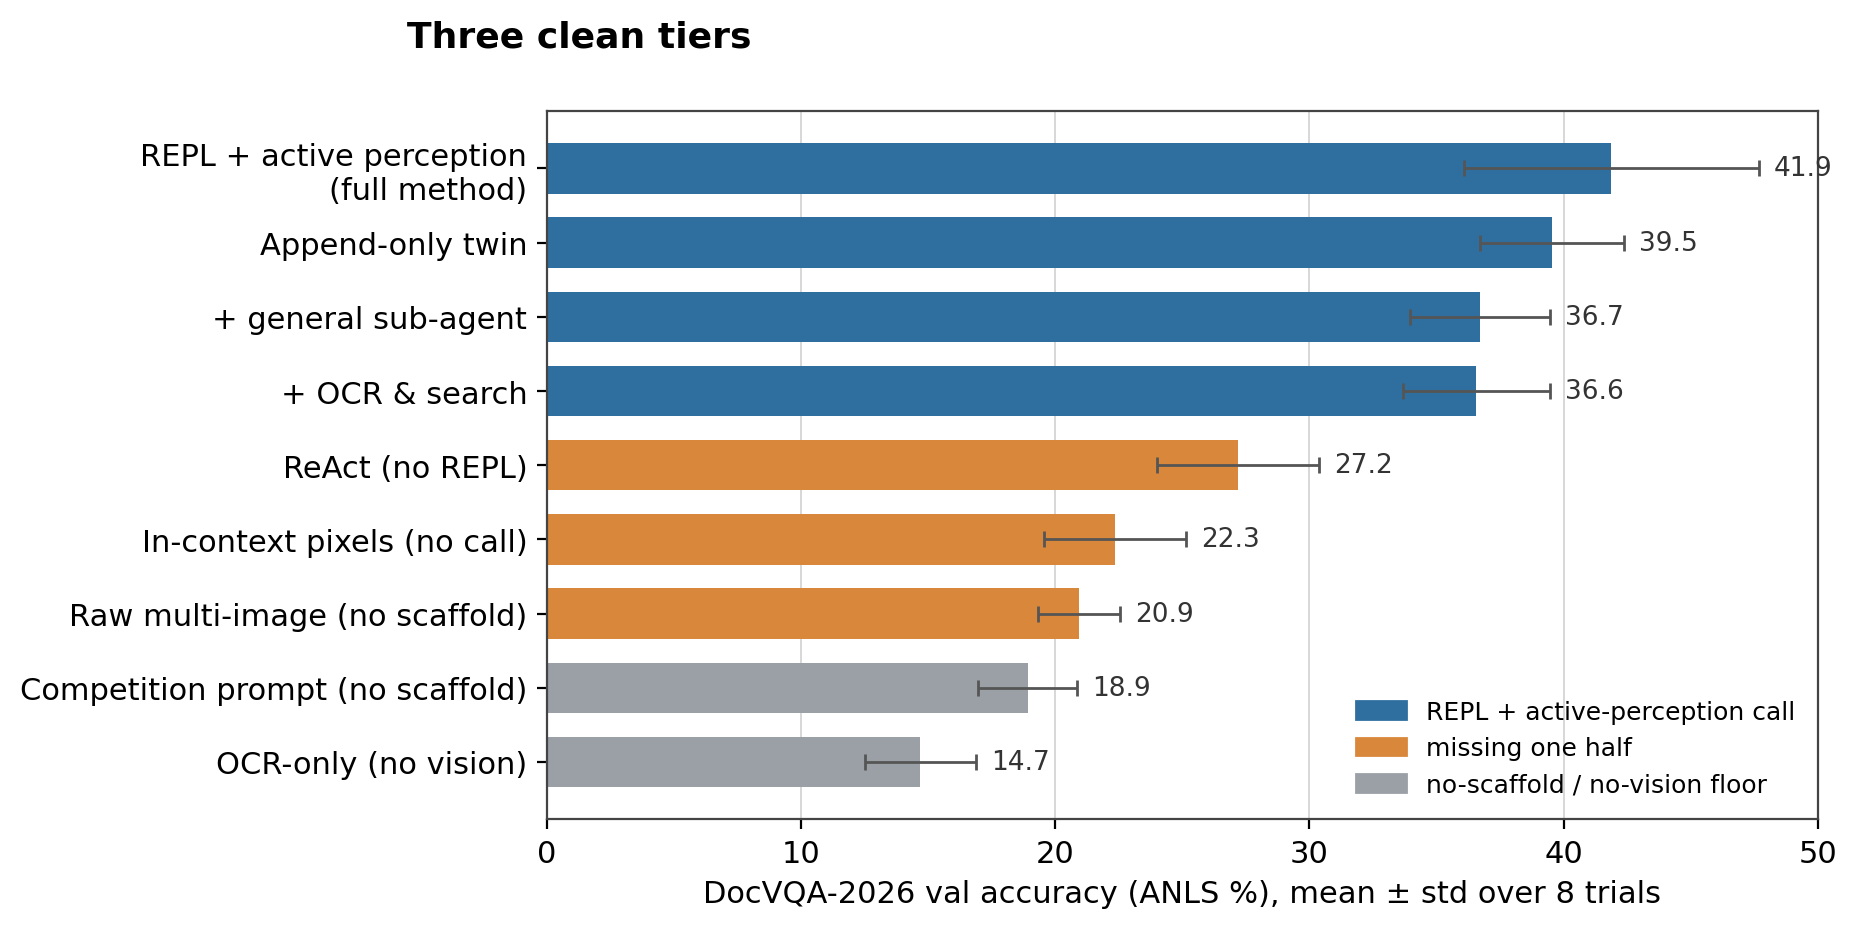
\includegraphics[width=0.9\linewidth]{figures/f3.png}\par}
\figcap{\textbf{Fig.~2.} Three clean tiers: REPL~+~perception ($\sim$36--42\%),
missing one half (21--27\%), OCR-only floor (15\%).}
\end{panel}

\begin{panel}{THE ADVANTAGE GROWS WITH LENGTH}
On short MP-DocVQA ($\le$20 pages) RLM leads the raw multi-image baseline by
\keyval{$\sim$4 pts}; on long MMLongBench-Doc ($\sim$47 pages) by
\keyval{$\sim$42 pts}. RLM stays flat across both --- it navigates the document
--- while the baseline's ``Unknown'' rate climbs from 22\% to 87\% as evidence
falls off a fixed page budget. On moderate DocVQA-2026 the edge comes instead
from \keyval{within-page density} (Fig.~4).
\end{panel}
\end{minipage}

\end{minipage}
\hfill
% =========================== RIGHT SIDEBAR (full height) ===========================
\begin{minipage}[t]{0.325\textwidth}\vspace{0pt}
\begin{panel}{BETTER EYES, OR A BETTER DIRECTOR?}
Swap the \keyval{actively driven VLM} for a \keyval{precomputed OCR channel}
(page text + figure captions + search). Same reasoner, REPL, and text
interface. It falls to \keyval{14.7\%}, the
study floor, with \keyval{0/10 in all 8 trials} on layout-bound categories
(drawings, maps). What collapses is not perception but \keyval{agency over it}:
question-blind reading cannot replace directed looks.

\vspace{5pt}
{\centering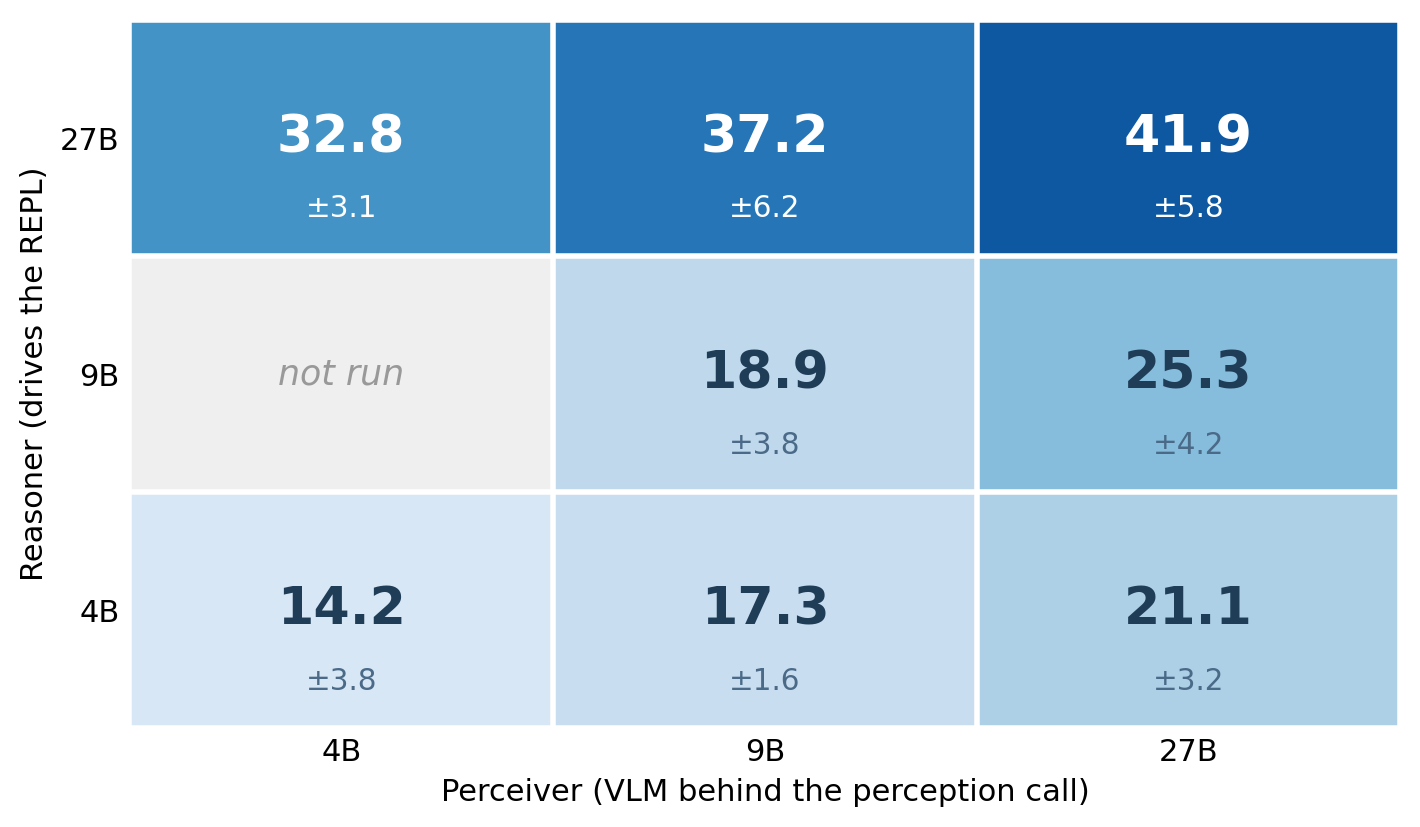
\includegraphics[width=0.88\linewidth]{figures/f5-matrix-poster.png}\par}
\figcap{\textbf{Fig.~3.} Reasoner $\times$ VLM matrix (val ANLS). Across a row
(better eyes) +6--9~pts; down a column (better reasoner) +21. A 27B reasoner
with 4B eyes (32.8) beats the reverse (21.1).}

\end{panel}

\begin{panel}{ADVANTAGE TRACKS VISUAL DENSITY}
{\centering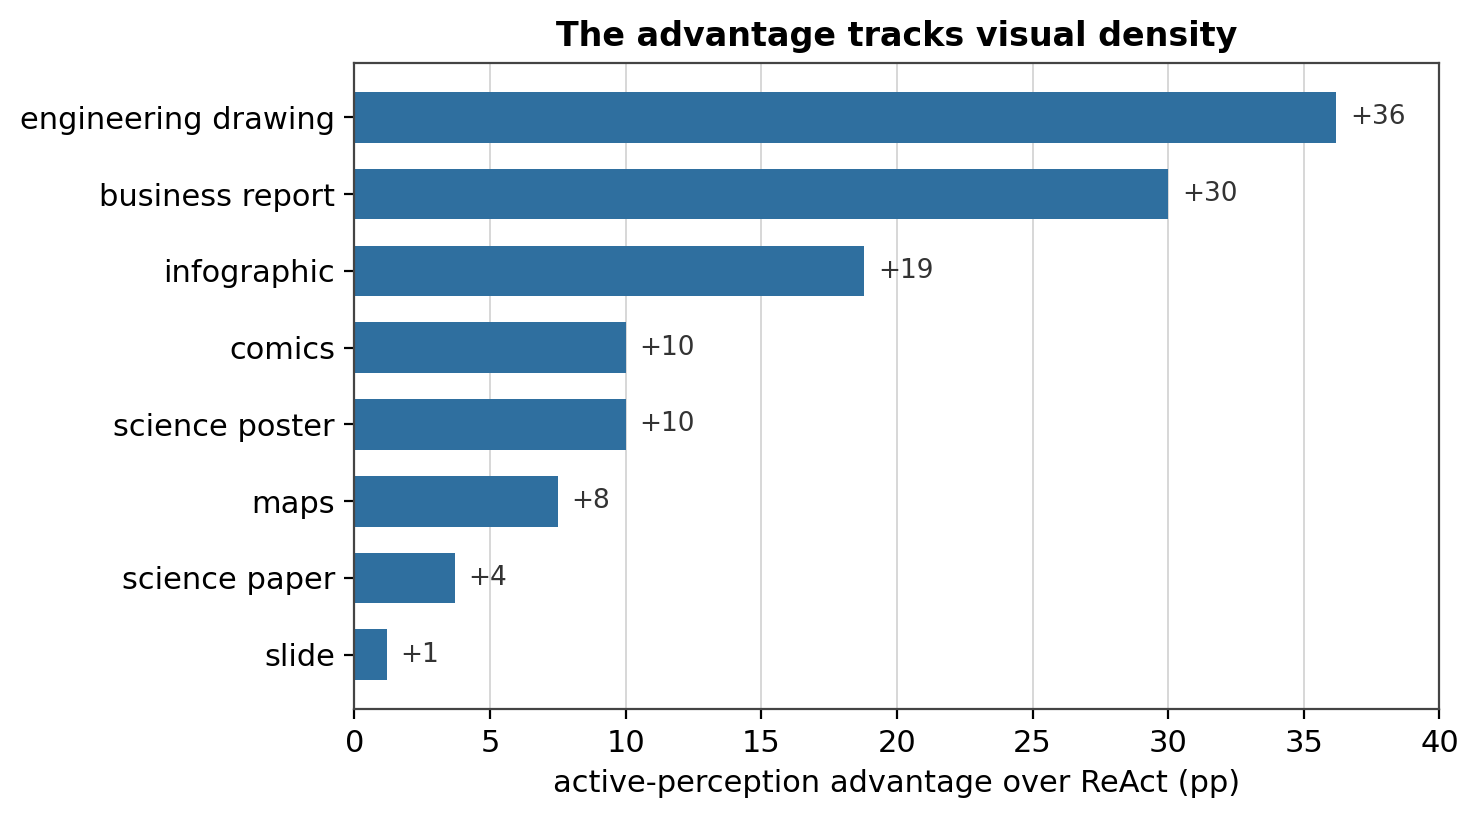
\includegraphics[width=0.95\linewidth]{figures/fcat.png}\par}
\figcap{\textbf{Fig.~4.} Advantage over ReAct (Yao et al., 2023) by category.
Largest on dense pages --- engineering drawings (+36), business reports (+30),
infographics (+19) --- smallest on text-linear ones: science papers (+4),
slides (+1).}
\end{panel}

\begin{panel}{LIMITATIONS}
\keyval{Generality costs calls} --- perception is a region at a time, each a
sequential VLM call ($\sim$13 steps/Q); unconstrained recursion can be ruinously
expensive (Borchmann et al., 2026). More steps mark a \emph{hard} document, not a
better answer. Cheap OCR retrieval or a smaller VLM behind the
call are open efficiency levers.

\vspace{4pt}
\keyval{And a floor}: the harness amplifies a strong-enough coder (31B Gemma:
+15~pts over ReAct) but cannot rescue one too weak to code (Gemma E4B collapses).
\end{panel}

\begin{panel}{OUTLOOK}
The REPL is a \keyval{symbolic substrate} for a neural model --- a medium to hold,
compose, and compute what its context cannot. That code helps at \emph{test time} is
established. The open question: could the symbolic substrate become \keyval{part of
the model itself} --- woven into how it learns and computes, not bolted on at
inference?

\vspace{4pt}
\keyval{The signal is there.} Over 8 trials the right answer is reached
\keyval{$\sim$69\%} of the time (oracle, pass@8) but reliably produced only
\keyval{$\sim$42\%} --- a 27-point gap a learning procedure could capture.

\vspace{7pt}
\begin{tcolorbox}[colback=white, colframe=pblue, boxrule=1.1pt, arc=5pt,
  left=9pt,right=9pt,top=6pt,bottom=6pt]
\begin{minipage}[c]{0.29\linewidth}

\includegraphics[width=\linewidth]{figures/qr.png}
\end{minipage}\hfill
\begin{minipage}[c]{0.65\linewidth}
{\raggedright \keyval{Full technical write-up}}\\[6pt]
{\smallfont \texttt{barisdeniz.is-a.dev}\\ \texttt{github.com/bdsaglam/docvqa}}
\end{minipage}
\end{tcolorbox}
\end{panel}

\begin{panel}{REFERENCES}
\reffont\justifying
Zhang, A.L., Kraska, T., Khattab, O. (2025). \emph{Recursive Language Models.}
arXiv:2512.24601.\\[2pt]
Wang, X. et al. (2024). \emph{Executable Code Actions Elicit Better LLM Agents
(CodeAct).} ICML.\\[2pt]
Yao, S. et al. (2023). \emph{ReAct: Synergizing Reasoning and Acting in LMs.}
ICLR.\\[2pt]
Gupta, T., Kembhavi, A. (2023). \emph{Visual Programming (VisProg).} CVPR.\\[2pt]
Surís, D., Menon, S., Vondrick, C. (2023). \emph{ViperGPT.} ICCV.\\[2pt]
Borchmann, Ł. et al. (2026). \emph{Strategic Navigation or Stochastic Search?
(MADQA).} arXiv:2603.12180.\\[2pt]
Mathew, M., Karatzas, D., Jawahar, C.V. (2021). \emph{DocVQA.} WACV.
\end{panel}
\end{minipage}

\end{document}
